\begin{figure}[htbp]
    \centering
    \subfigure[Tela de login. \label{fig:login}]{
        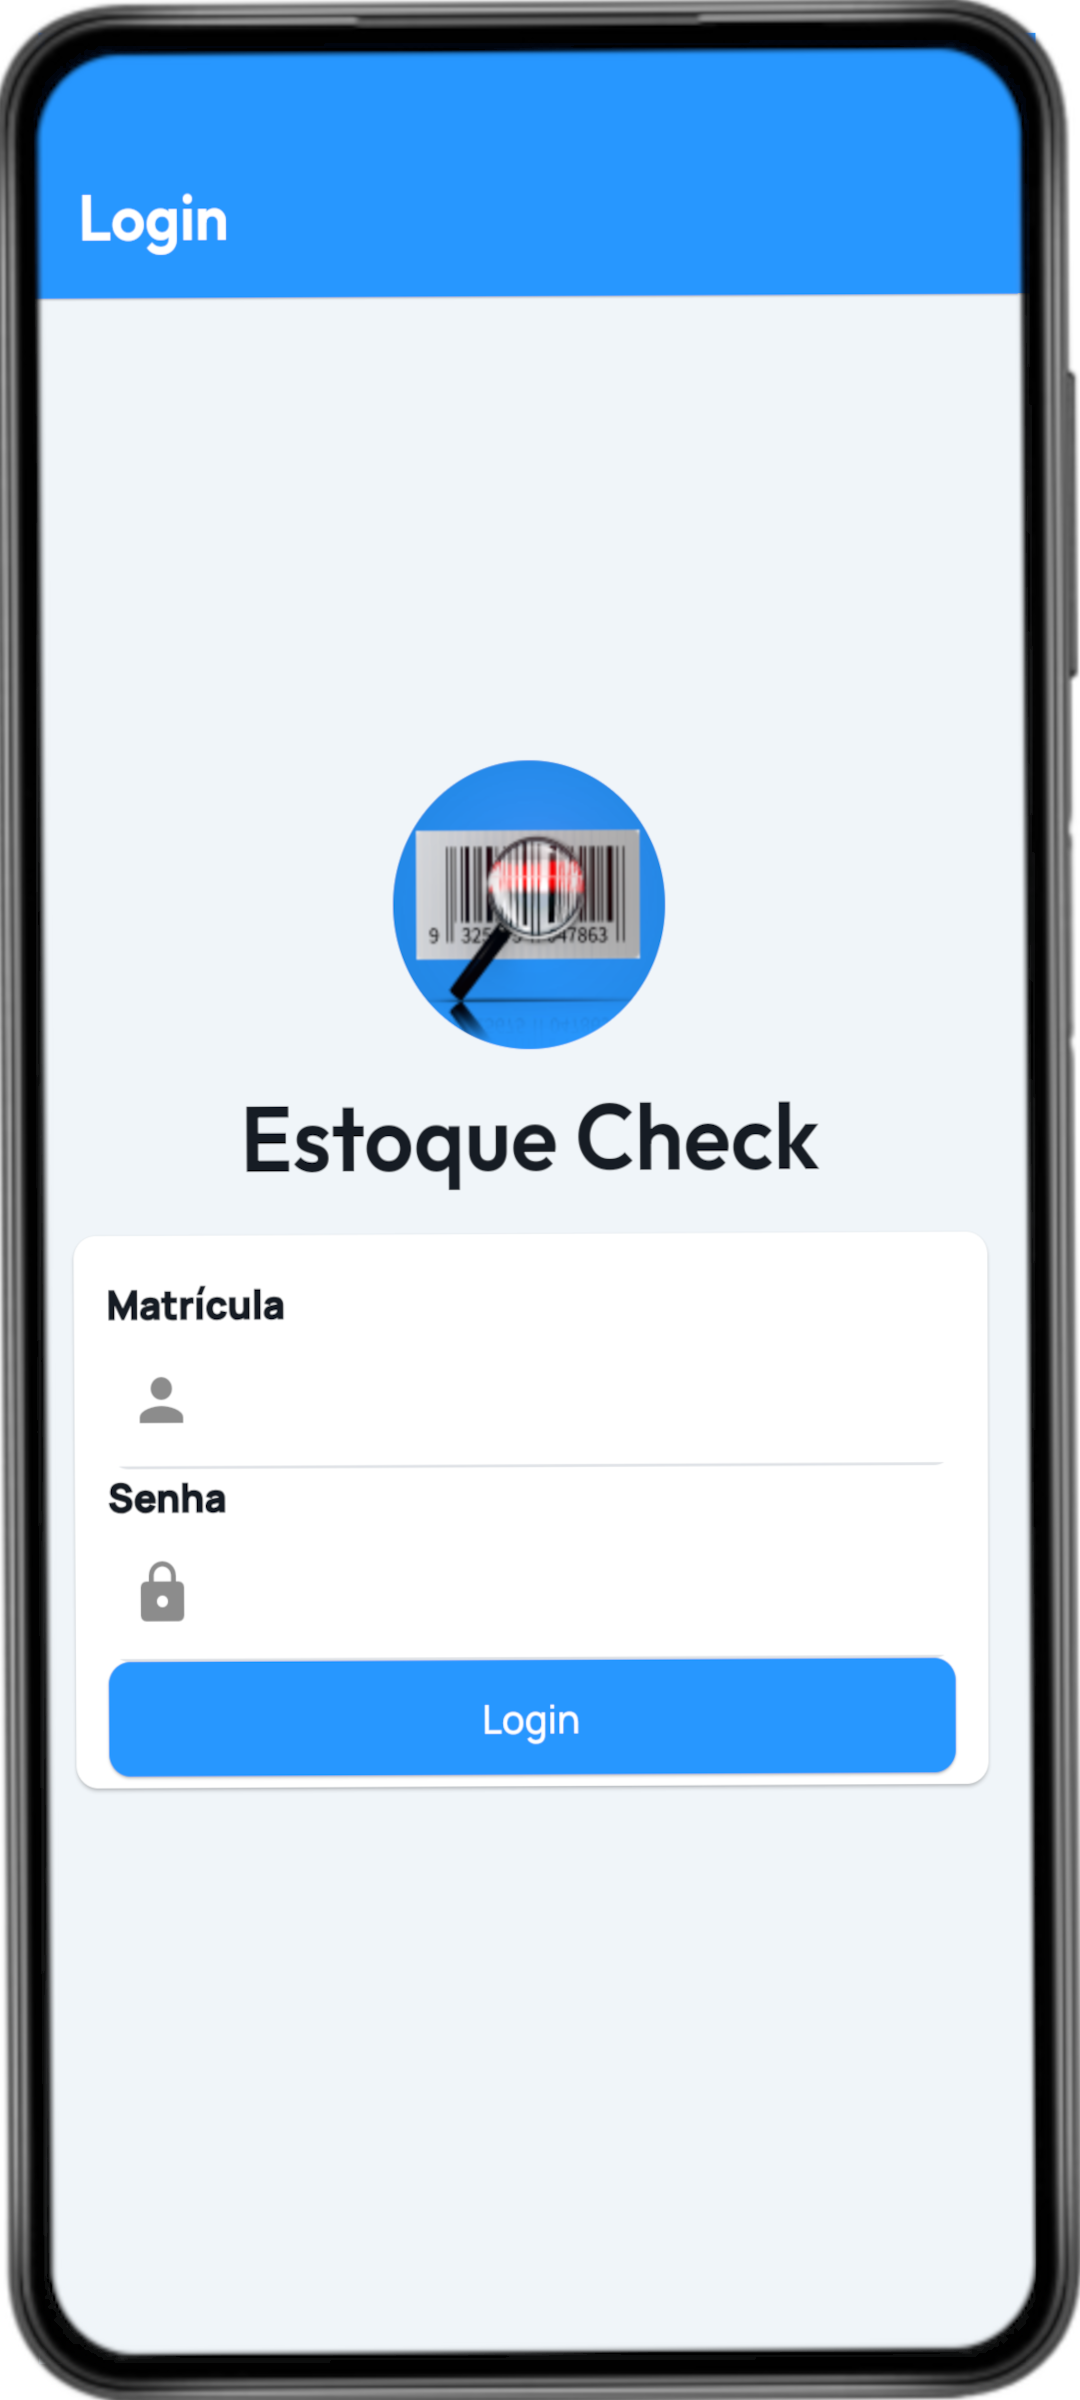
\includegraphics[width=0.22\textwidth]{imgs/login.png}
    }
    \quad
    \subfigure[Tela principal. \label{fig:homepage}]{
        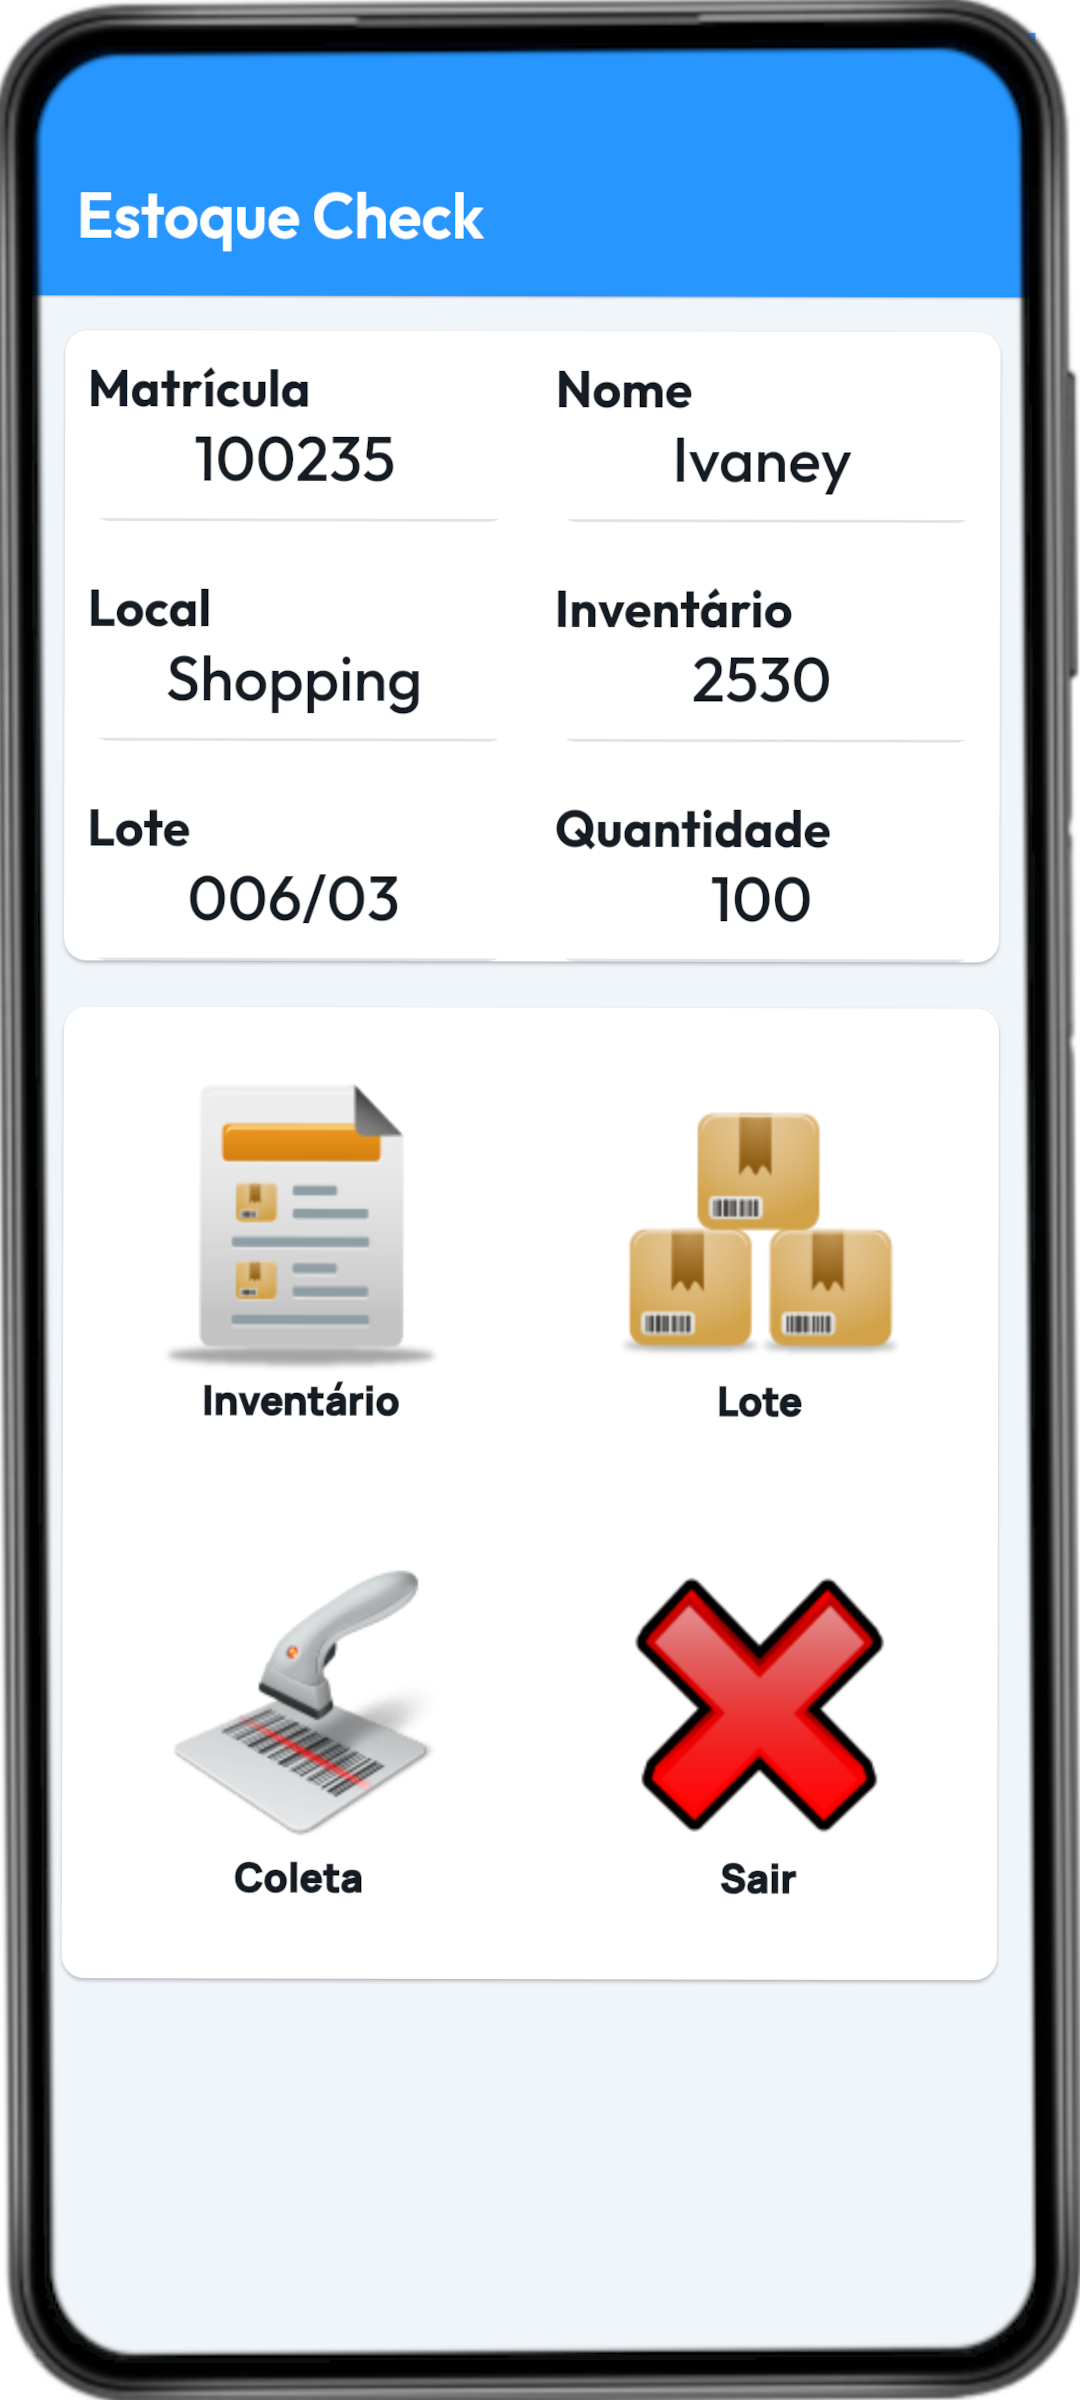
\includegraphics[width=0.22\textwidth]{imgs/homepage.png}
    }
    \quad
    \subfigure[Seleção de inventário.\label{fig:inventario}]{
        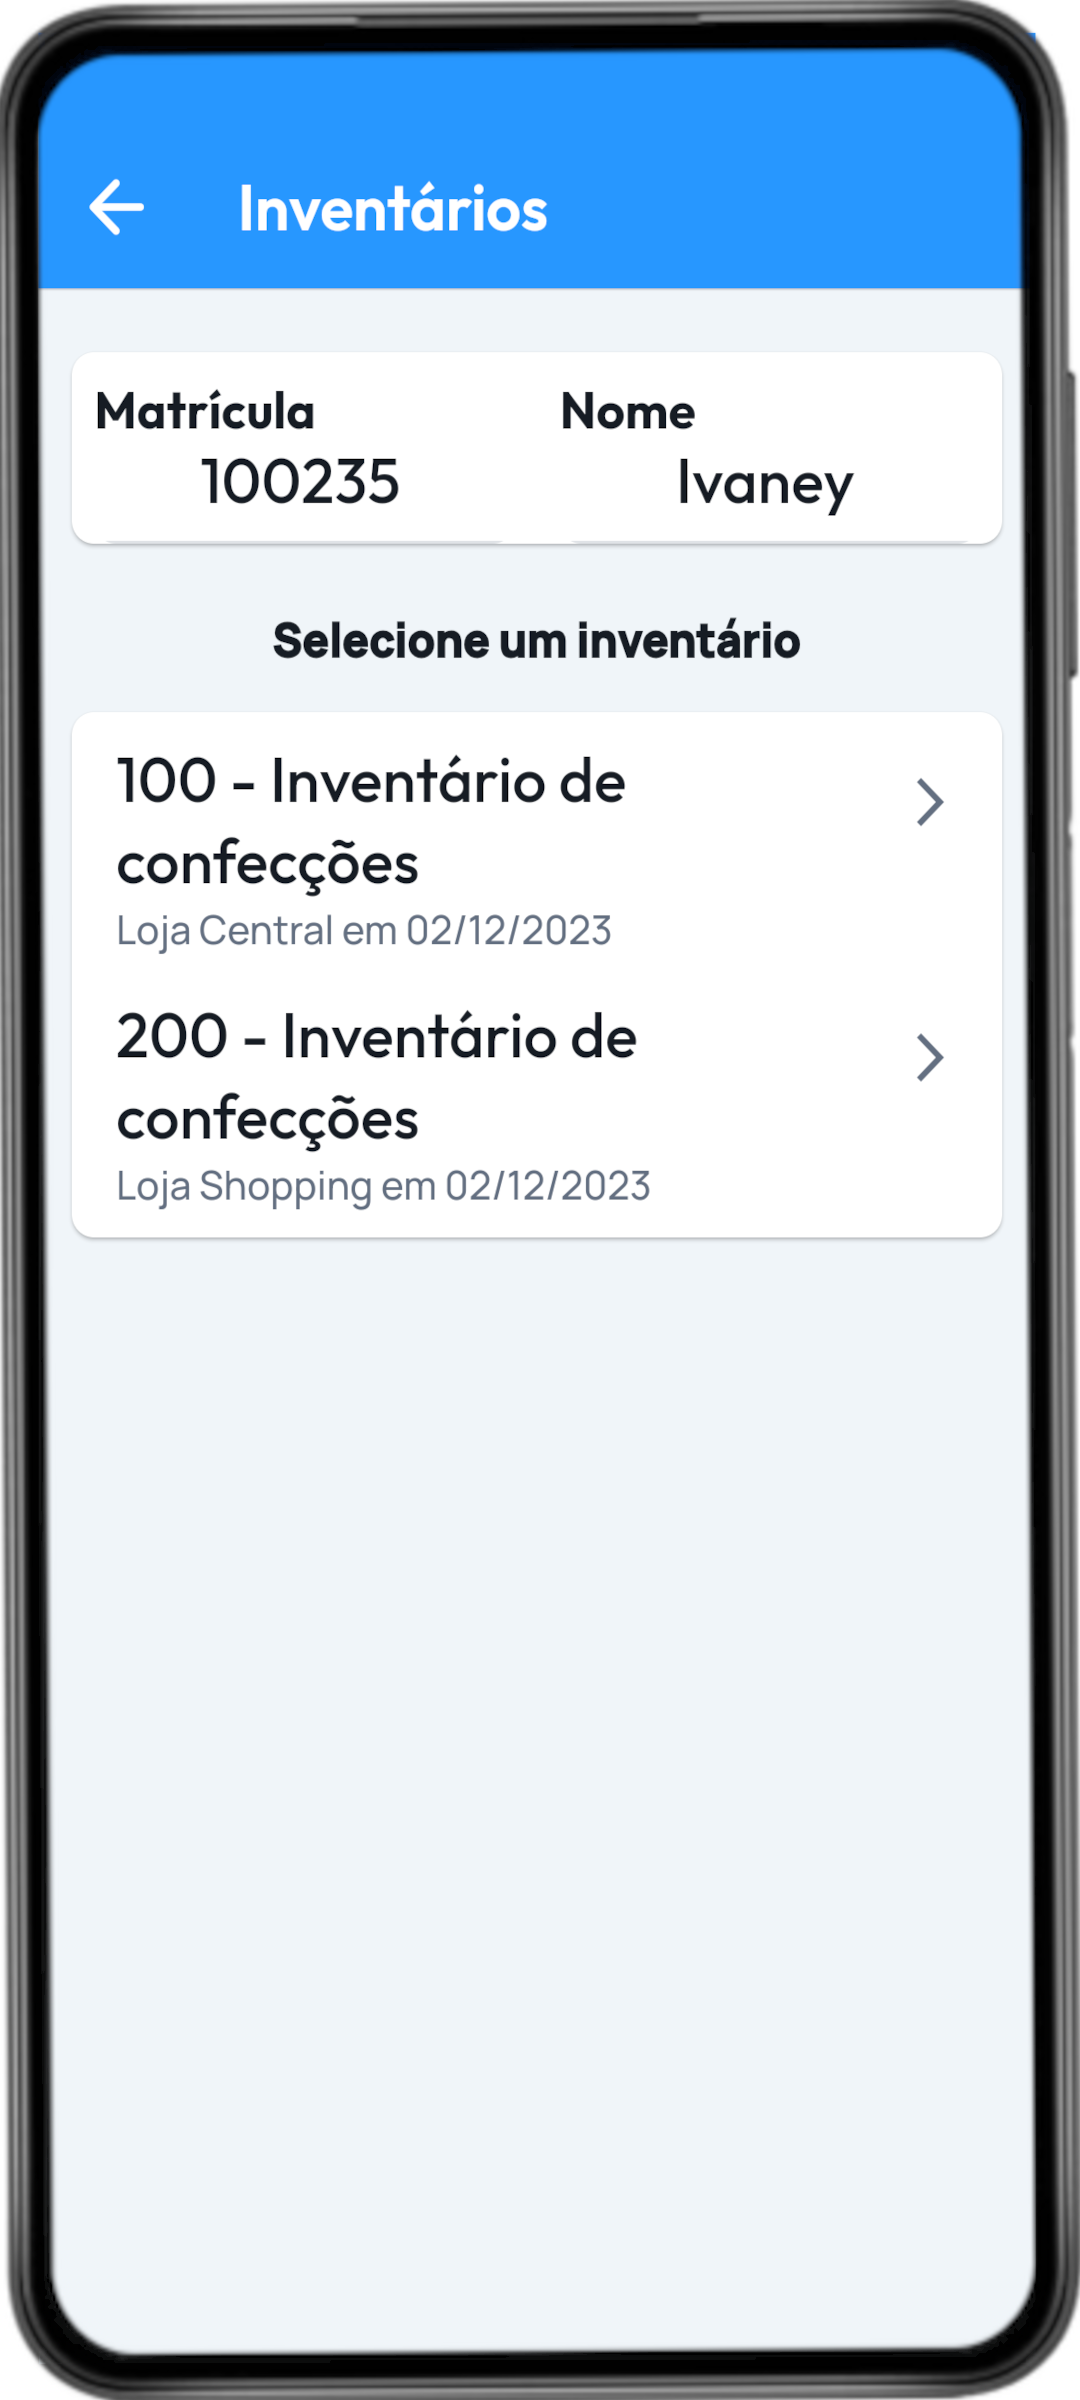
\includegraphics[width=0.22\textwidth]{imgs/inventario.png}
    }
    \quad
    \subfigure[Seleção de Lote.\label{fig:lote}]{
        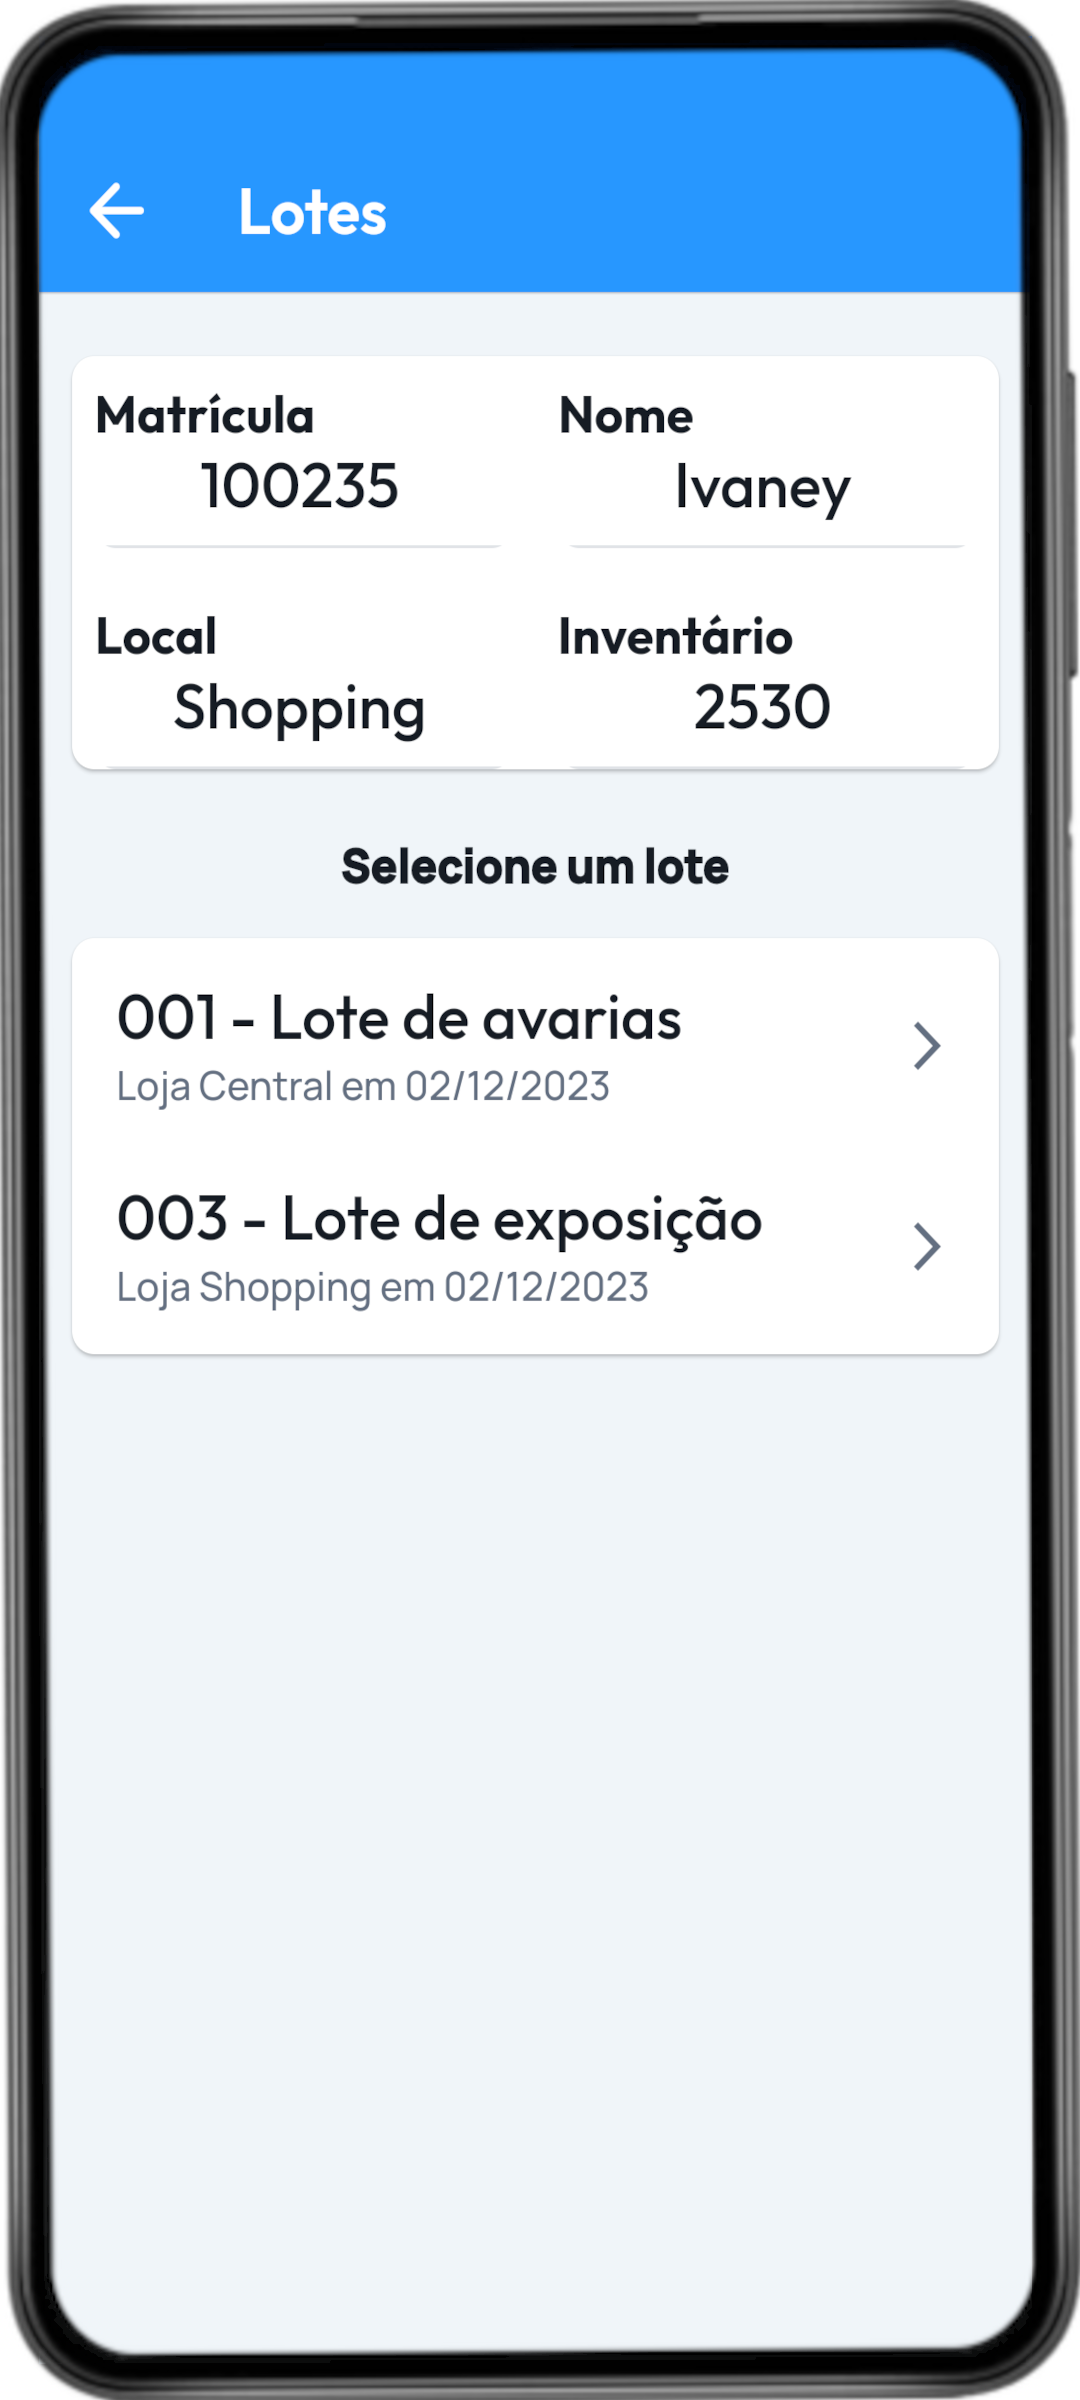
\includegraphics[width=0.22\textwidth]{imgs/lote.png}
    }
    \quad
    \subfigure[Coleta para contagem.\label{fig:coleta}]{
        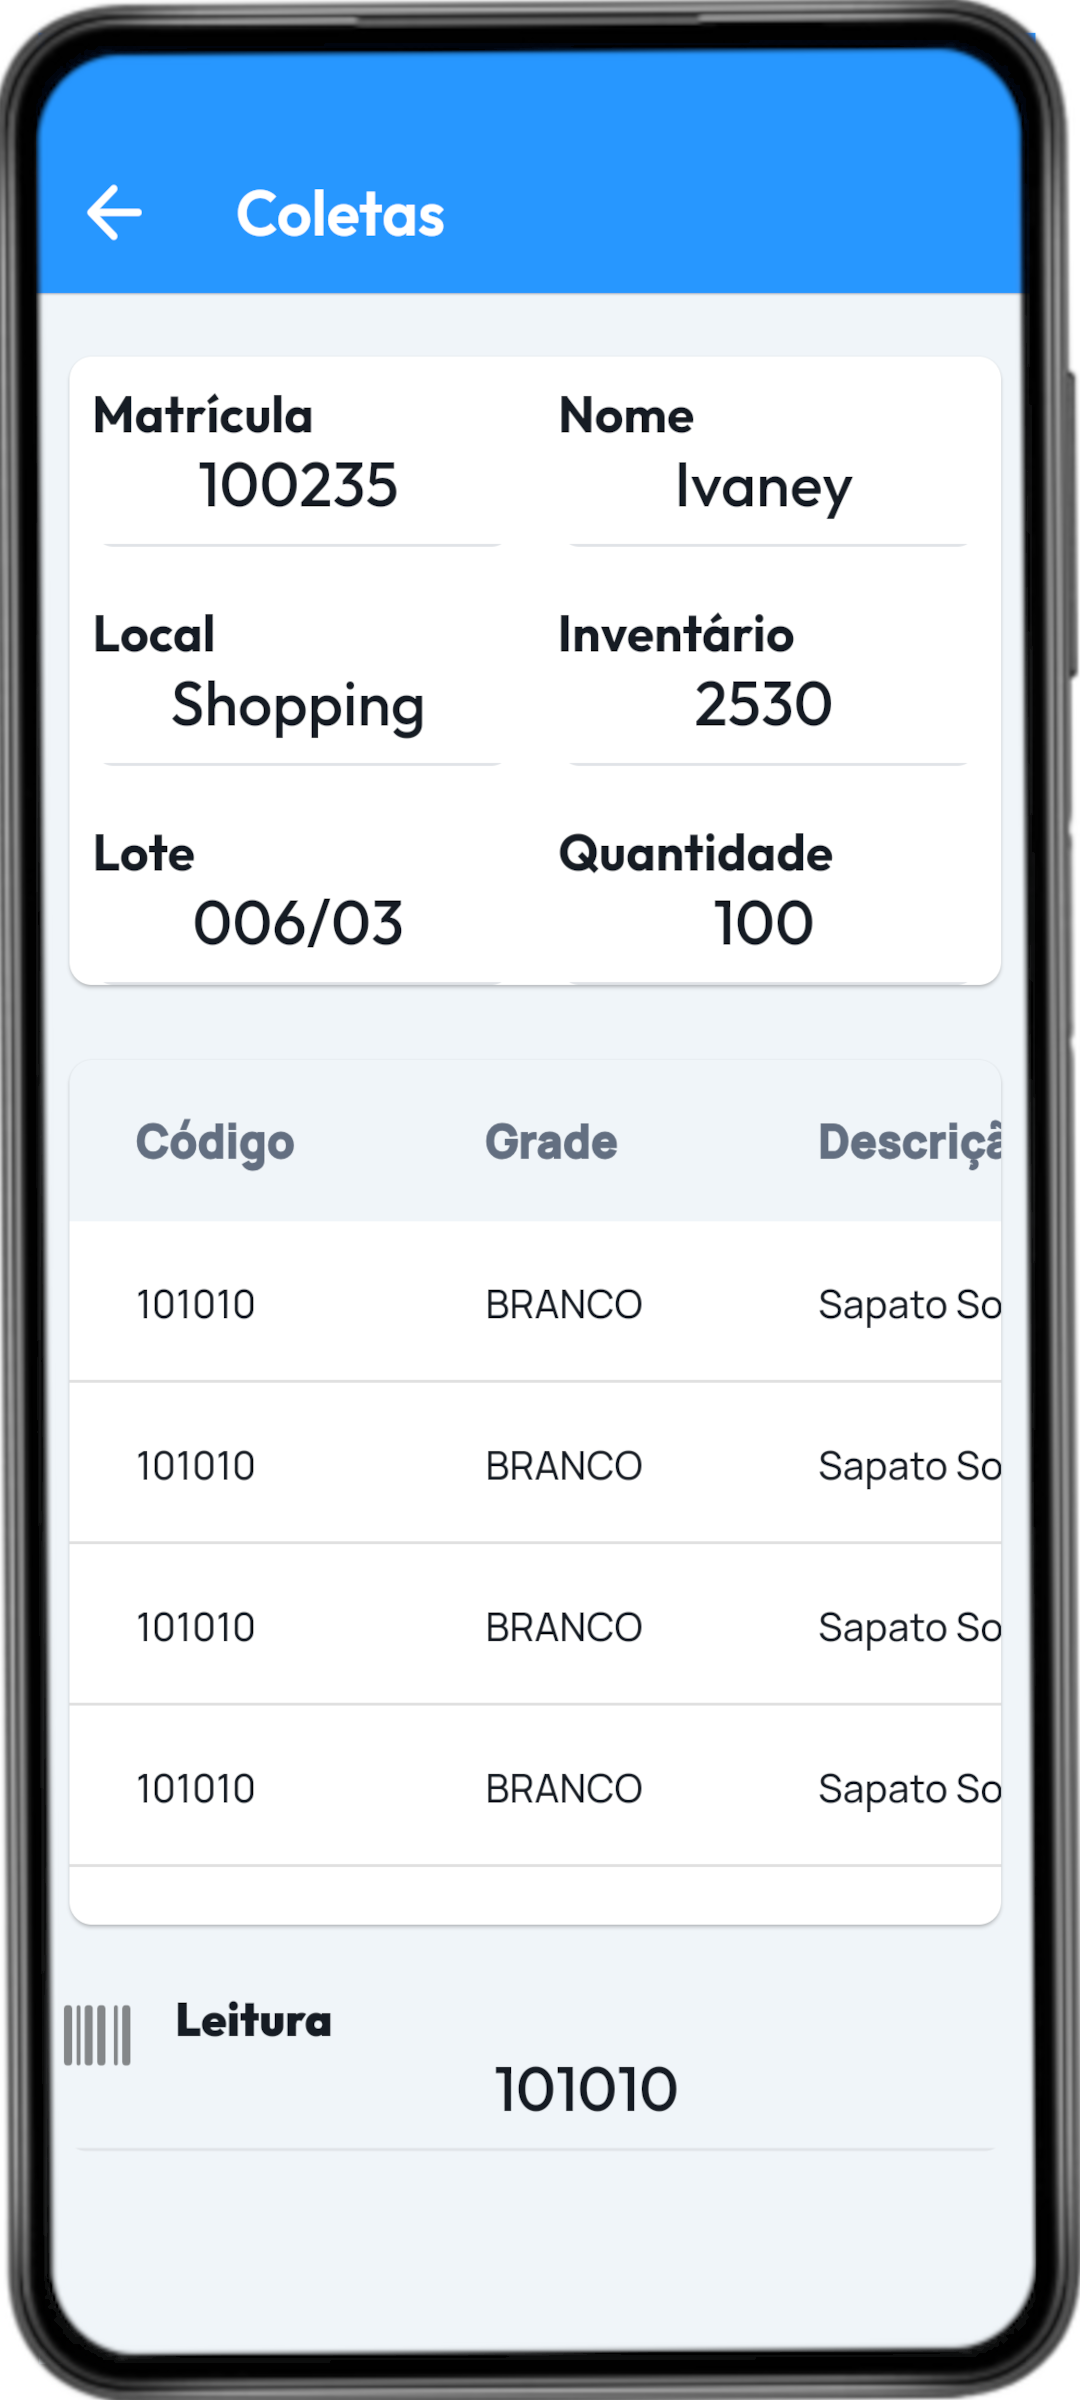
\includegraphics[width=0.22\textwidth]{imgs/coleta.png}
    }
    \label{fig:grupo01}
    \caption{Layout de telas para o aplicativo}
\end{figure}

No mercado brasileiro, existem diversos aplicativos para contagem de inventário em coletores Android, cada um com suas vantagens e desvantagens:

\begin{itemize}
    \item IS Collector
    \begin{itemize}
        \item Trabalho online e offline: Permite contagem mesmo sem internet, com sincronização posterior.
        \item Leitura por código de barras e câmera: Flexibilidade para diferentes tipos de inventário.
        \item Modos de trabalho abrangentes: Coletas avulsas, inventários completos e conferências.
        \item Visualização de descrição do item: Informação adicional durante a leitura.
        \item Site: https://iscollector.com.br/
    \end{itemize}
    \item KCollector
    \begin{itemize}
        \item Transforma o celular em um coletor: Solução acessível e prática.
        \item Automação de processos: Otimiza o fluxo de trabalho e reduz custos.
        \item Ideal para diversos segmentos: Indústrias, supermercados, farmácias, lojas de varejo em geral.
        \item Site: https://www.kcollector.com.br/
    \end{itemize}
    \item Stock e Inventário Simples
    \begin{itemize}
        \item Facilidade de uso: Ideal para iniciantes e pequenos negócios.
        \item Gerenciamento de estoque completo: Controle de entrada e saída de produtos, datas de validade, lotes e mais.
        \item Integração com Excel: Importação e exportação de dados para análise.
        \item Site: https://chester-sw.com/
    \end{itemize}
\end{itemize}



